\documentclass{lehramt-informatik-haupt}
\liLadePakete{syntax}
\begin{document}

%%%%%%%%%%%%%%%%%%%%%%%%%%%%%%%%%%%%%%%%%%%%%%%%%%%%%%%%%%%%%%%%%%%%%%%%
% Theorie-Teil
%%%%%%%%%%%%%%%%%%%%%%%%%%%%%%%%%%%%%%%%%%%%%%%%%%%%%%%%%%%%%%%%%%%%%%%%

\chapter{Struktogramm}

Software zum Erstellen von Struktogrammen:
\url{https://github.com/fesch/Structorizer.Desktop}

\cite[Seite 13-14]{oomup:fs:3}

\section{Aufgaben}

\cite{net:html:pns-berlin:uebung-1}

\begin{enumerate}

%%
%
%%

\item Zeichne ein Struktogramm zu folgender Aufgabe und gib eine
Implementierung an.

Die Methode \verb|anzeigen(int i)| verringert die Zahl \verb|i|
schrittweise um \verb|10| und gibt dabei jeweils den Buchstaben
„\verb|z|“ (zweistellig (oder mehr)) auf dem Bildschirm aus, bis
\verb|i| kleiner als \verb|10| ist.

Die nun einstellige Zahl \verb|i| wird entsprechend um jeweils \verb|1|
verkleinert und der Buchstabe „\verb|e|“ (einstellig) ausgegeben, bis
man schließlich bei Null angelangt ist.

\begin{liAntwort}
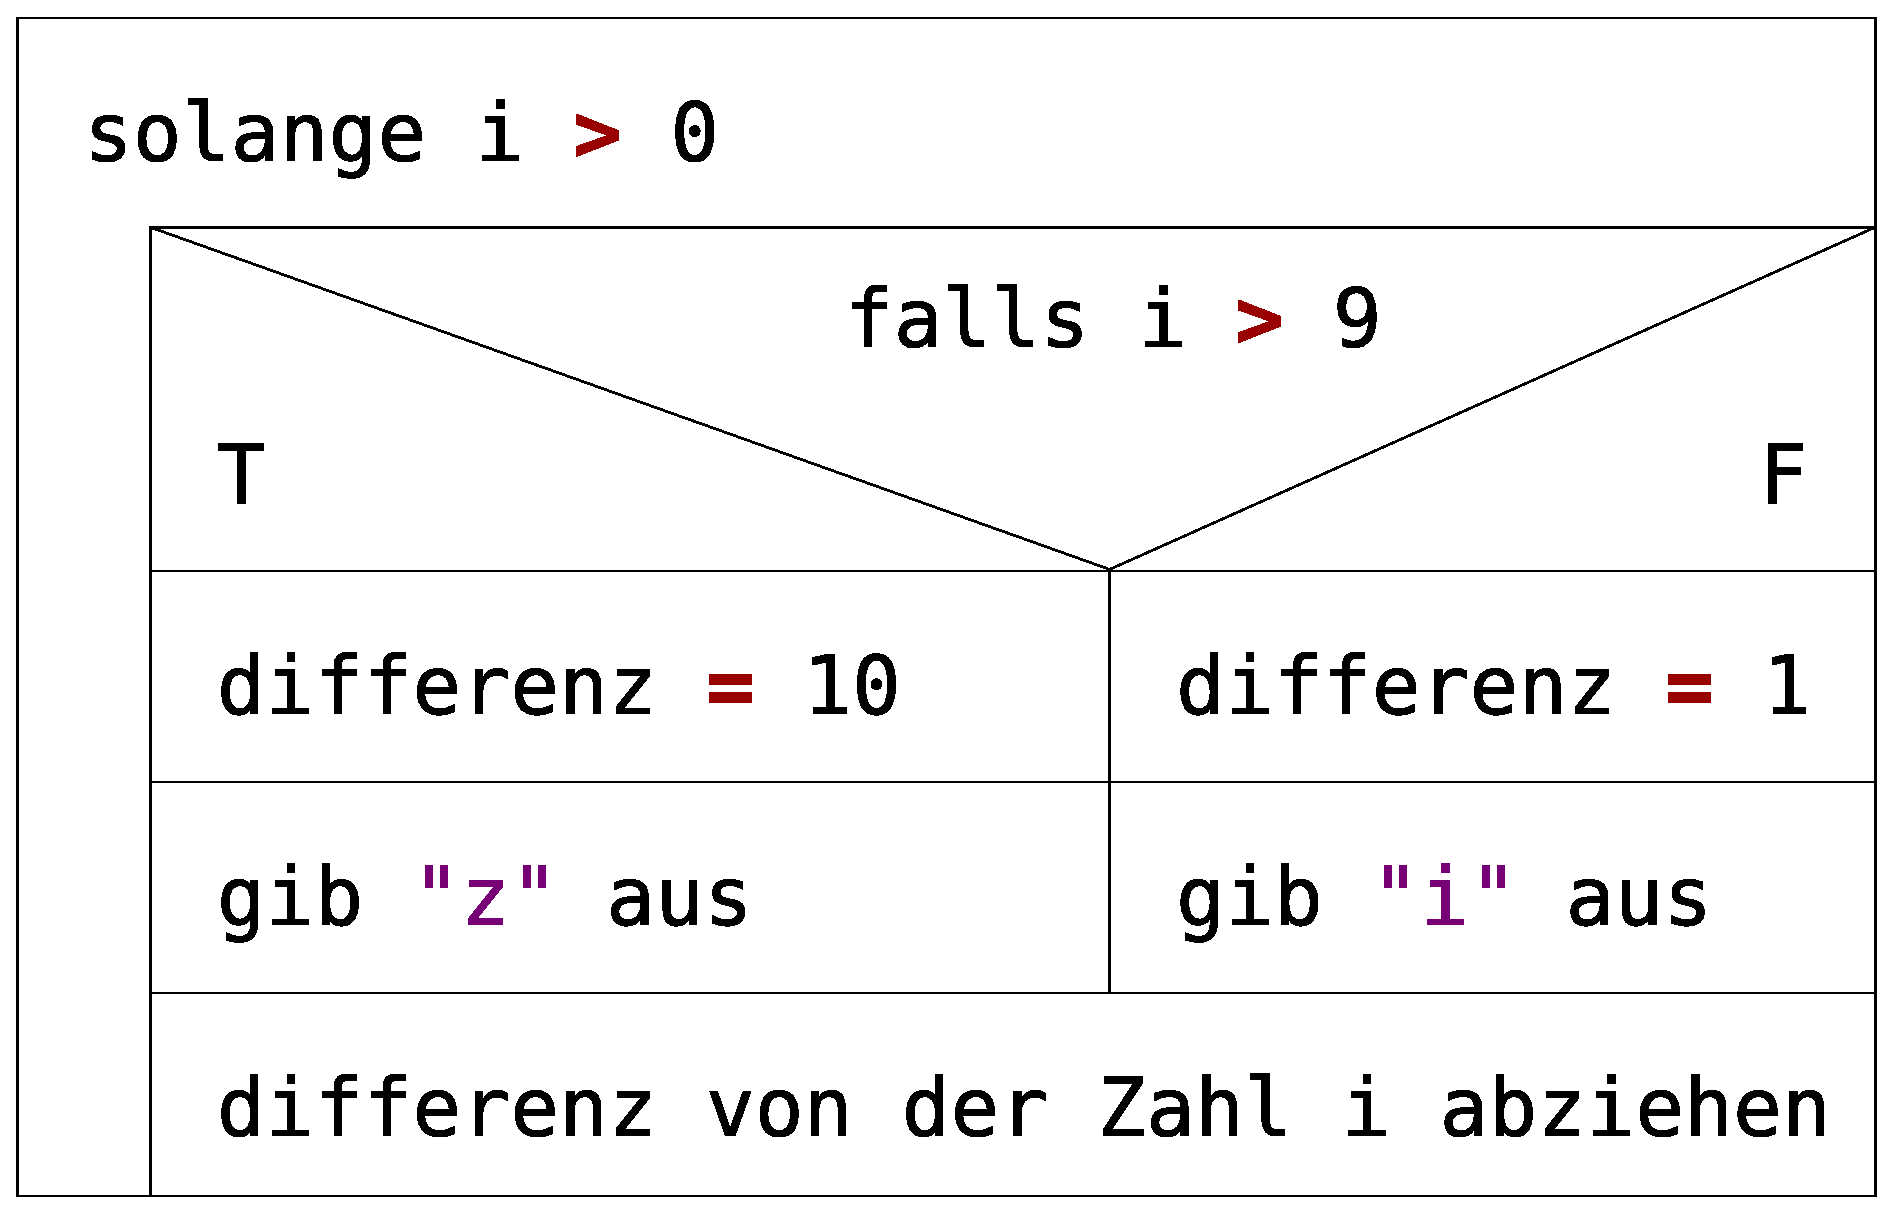
\includegraphics[width=0.7\linewidth]{Aufgabe-1.eps}

\begin{minted}{java}
public void anzeigen(int i) {
  int differenz;
  while (i > 0) {
    if (i > 9) {
      differenz = 10;
      System.out.print("z");
    } else {
      differenz = 1;
      System.out.print("e");
    }
    i = i - differenz;
  }
}
\end{minted}
\end{liAntwort}

%%
%
%%

\item Beschreibe, was die folgende Methode auf dem Bildschirm ausgibt,
wenn für \verb|a = 5| und für \verb|b = 12| übergeben wird. Zeichne das
zugehörende Struktogramm.

\begin{minted}{java}
public void ausgabe(int a, int b) {
  int x = a;
  while (x <= b)
  {
    y = x * x - 2;
    System.out.prinln(x + ".." + y);
    x = x + 3;
  }
}
\end{minted}

\begin{liAntwort}
\begin{verbatim}
5..23
8..62
11..119
\end{verbatim}

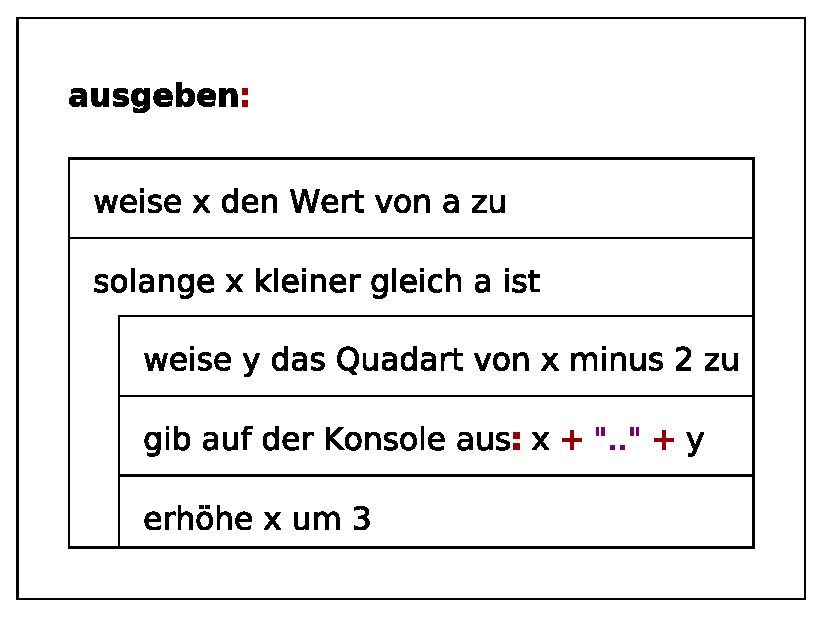
\includegraphics[width=0.7\linewidth]{Aufgabe-2.eps}
\end{liAntwort}

%%
%
%%

\item Firma \emph{OnlyOne} verkauft nur einen Artikel. Für diesen
Artikel hat ein Programmierer eine Methode geschrieben, mit der man aus
der Kundenummer und der gewünschten Anzahl den Endpreis berechnen kann.

Zeichne für die folgende Beschreibung das zugehörige Struktogramm und
gib eine Implementierung in Java an.

\begin{minted}{java}
public double preis(int knr, int anzahl)
{
    ...
}
\end{minted}

Wenn es sich um einen \emph{Stammkunden} (knr = 1..999) handelt, dann
erhält der Kunde die Waren zu einem Stückpreis von \emph{52.- €}. Alle
anderen Kunden zahlen \emph{58.- €} pro Stück.

Bei Bestellungen von \emph{mehr als 20} Stück wird jeweils ein
Mengenrabatt von \emph{5 \%} gewährt.

Das Programm gibt den Gesamtpreis der gewünschten Waren zurück.

\begin{liAntwort}
\begin{minted}{java}
public void preis(int knr, int anzahl) {
  double preis;
  if (knr > 0 && knr < 1000) {
    preis = 52;
  }
  else {
    preis = 58;
  }
  if (anzahl > 20) {
    preis = 0.95 * preis;
  }
  System.out.println("Preis=" + (anzahl * preis));
}
\end{minted}

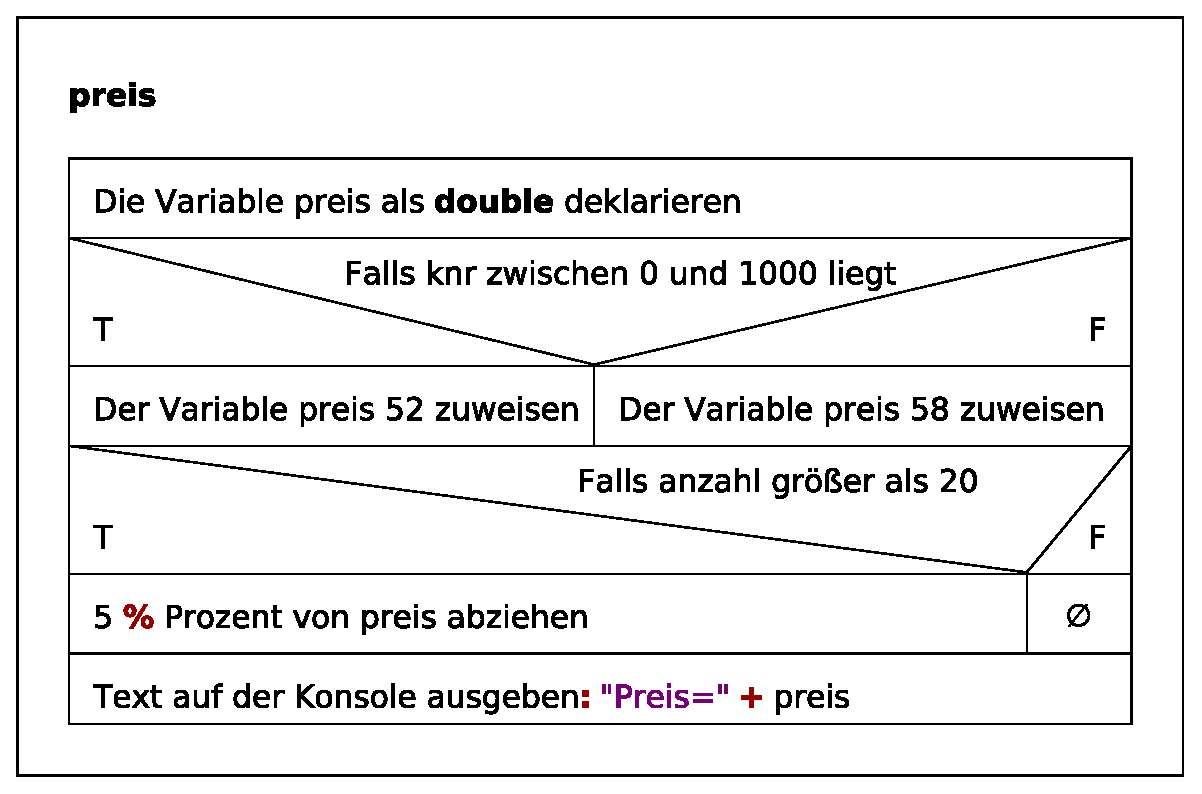
\includegraphics[width=0.7\linewidth]{Aufgabe-3.eps}
\end{liAntwort}

\end{enumerate}

\literatur
\end{document}
